%% ****** Start of file apstemplate.tex ****** %
%%
%%
%%   This file is part of the APS files in the REVTeX 4.2 distribution.%%
%%   Copyright (c) 2024 The American Physical Society.
%%
%%   See the REVTeX 4 README file for restrictions and more information.
%%
%
% This is a template for producing manuscripts for use with REVTEX 4.2
% Copy this file to another name and then work on that file.
% That way, you always have this original template file to use.
%
% Group addresses by affiliation; use superscriptaddress for long
% author lists, or if there are many overlapping affiliations.
%  N.B. The groupedaddress option will reorder the author list based
%  on the order in which affiliations appear. Please be sure to check the author 
%  order. You can also use the unsortedaddress(?) option instead to prevent that
%  behavior.
% For Phys. Rev. appearance, change preprint to twocolumn.
% Choose physrev, prl, or rmp for journal
%  N.B. physrev is appropriate for all APS journals except prl and rmp
%  Add 'draft' option to mark overfull boxes with black boxes
%  Add 'showkeys' option to make keywords appear
%\\documentclass[aps,physrev,preprint,groupedaddress]{revtex4-2}
\documentclass[aps,physrev,twocolumn,superscriptaddress]{revtex4-2}
%\documentclass[aps,prl,preprint,superscriptaddress]{revtex4-2}
%\documentclass[aps,prl,reprint,groupedaddress]{revtex4-2}
%\documentclass[aps,rmp,preprint,superscriptaddress]{revtex4-2}
%\documentclass[aps,rmp,reprint,groupedaddress]{revtex4-2}

% You should use BibTeX and apsrev.bst for references
% Choosing a journal automatically selects the correct APS
% BibTeX style file (bst file), so only uncomment the line
% below if necessary.
%\bibliographystyle{apsrev4-2}


\usepackage{graphicx}%
\usepackage{multirow}%
\usepackage{amsmath,amssymb,amsfonts}%
\usepackage{amsthm}%
\usepackage{mathrsfs}%
\usepackage{xcolor}%
\usepackage{textcomp}%
\usepackage{booktabs}%
\usepackage{listings}%
\usepackage{todonotes}
\usepackage{lineno}
\usepackage{xspace}

\begin{document}

\include{macro}
%\include{checklist}
% Use the \preprint command to place your local institutional report
% number in the upper righthand corner of the title page in preprint mode.
% Multiple \preprint commands are allowed.
% Use the 'preprintnumbers' class option to override journal defaults
% to display numbers if necessary
%\preprint{}

%Title of paper
\title{Track Finding and Particle Identification Performance with Particle Physics Foundation Models}

% repeat the \author .. \affiliation  etc. as needed
% \email, \thanks, \homepage, \altaffiliation all apply to the current
% author. Explanatory text should go in the []'s, actual e-mail
% address or url should go in the {}'s for \email and \homepage.
% Please use the appropriate macro foreach each type of information

% \affiliation command applies to all authors since the last
% \affiliation command. The \affiliation command should follow the
% other information
% \affiliation can be followed by \email, \homepage, \thanks as well.
\author{}
%\email[]{Your e-mail address}
%\homepage[]{Your web page}
%\thanks{}
%\altaffiliation{}
\affiliation{Brookhaven National Laboratory}
\affiliation{Columbia University}

%Collaboration name if desired (requires use of superscriptaddress
%option in \documentclass). \noaffiliation is required (may also be
%used with the \author command).
%\collaboration can be followed by \email, \homepage, \thanks as well.
%\collaboration{}
%\noaffiliation

\date{\today}

\begin{abstract}
Modern high energy nuclear and particle physics experiments produce large amounts of sparse data that must be reduced significantly in size before performing physics analysis. Recently, there has been an effort to evaluate Foundation Models as a potential tool for performing data analysis. These models have been shown to learn features in high dimensional datasets based on the multi-modal data they are trained on. To show their effectiveness at performing complex pattern recognition tasks, such as reconstructing charged particles in a magnetic field, we evaluated the performance of a Foundation Model based reconstruction on several downstream tasks with a dataset composed of spacepoints in a Time Projection Chamber. We show that the performance of the Foundation Model based data analysis significantly improves upon that of traditional methods, and furthermore can be adapted to learn additional tasks that are not necessarily related to the initial training objective.
\end{abstract}



%\maketitle must follow title, authors, abstract, and keywords
\maketitle

\linenumbers

% body of paper here - Use proper section commands
% References should be done using the \cite, \ref, and \label commands

\section{Introduction}
Data reconstruction for high energy nuclear and particle physics experiments is becoming increasingly challenging as modern and future facilities deliver ever higher luminosities. At the Relativistic Heavy Ion Collider, the sPHENIX experiment operates with a streaming readout data acquisition at rates far beyond those of previous generations of RHIC detectors, while the High-Luminosity Large Hadron Collider and the future Electron-Ion Collider will present comparable or greater demands, which increase the detector occupancies. Consequently, there has been significant effort in exploring new technologies to maintain high physics performance.   

In artificial intelligence (AI) research, the emergence of large language models has marked a major shift in model development, moving from specialized architectures designed for a single task toward general architectures adaptable to many tasks~\cite{Vaswani:2017}. Foundation models (FMs) are pretrained on large datasets to learn general representations, and are subsequently adapted to a wide variety of downstream tasks through lightweight fine-tuning or small task-specific adapters.  
Their ability to use self-supervised learning is particularly attractive for nuclear and particle physics, where unlabeled experimental data are abundant while fully labeled simulated data are computationally expensive and carry their own modeling uncertainties.

There has been a growing research effort into utilizing FMs for nuclear and particle physics, with much of the development targeting jet physics, since jets can be represented as ordered sets of constituents that resemble the token sequences of language models. Models pretrained on large jet-constituent datasets have been adapted to classification, generation, regression, reweighting, unfolding, and anomaly detection within a single framework~\cite{Birk:2024OmniJet,Golling:2024MPM,Harris:2025RS3L,Mikuni:2025OmniLearn,Bhimji:2026OmniLearned}. FMs have also been applied to calorimeter simulation~\cite{CardonaGiraldo:2026Calorimetry} and to cross-domain transfer from collider jets to neutrino interactions~\cite{Krzmanc:2026CrossDomain}, the latter demonstrating that learned representations can survive a change of both experiment and physics process. Most of these studies operate on high-level or partially reconstructed inputs, including jet constituents, particle-flow candidates, and four-vectors, which are themselves produced by conventional reconstruction chains. At a lower reconstruction level, Ref.~\cite{Giroux:2026ReadoutFM} introduces a proto-FM operating directly on the pixel and timing readout of an imaging Cherenkov detector, fine-tuned for particle identification and noise filtering, although its inputs are hit sequences already associated with a single track.

Substantial effort has also been devoted to machine learning (ML)-based charged-particle tracking, largely motivated by the TrackML challenges~\cite{Amrouche:2023TrackMLThroughput}. Graph neural networks, in which detector hits are treated as nodes and candidate track segments as edges, have been developed for this task, including Exa.TrkX~\cite{Ju:2021} and EggNet~\cite{Calafiura:2024}. Transformer-based~\cite{Miao:2024} and state-space-model-based~\cite{Jiang:2025} tracking approaches have also been explored. Related ML methods, including MLPF~\cite{Pata:2021MLPF} and HGPflow~\cite{Kakati:2025HGPflow}, perform particle-flow reconstruction by combining reconstructed tracks with calorimeter information. Although these models can achieve strong performance, most are optimized for a particular reconstruction objective using task-specific labeled samples.

The Foundation Model for Nuclear and Particle Physics (FM4NPP)~\cite{Park:2025FM4NPP} is a pretrained model designed to learn transferable representations from low-level detector data through self-supervised learning and to support multiple downstream reconstruction tasks. It is pretrained on spacepoints from the sPHENIX Time Projection Chamber (TPC)~\cite{Li:2026TPCpp10M}. In this work, we evaluate FM4NPP on several tracking-related downstream tasks and compare its performance with conventional reconstruction algorithms.

%There has been a growing research effort into utilizing FMs for nuclear and particle physics. FMs are being explored at all levels of data analysis, for example with jets~\cite{Krzmanc:2026fdw, Bhimji:2025isp}, calorimetry material modeling~\cite{Cardona-Giraldo:2026rnn}, DIRC reconstruction~\cite{Giroux:2025elr}, and more. 

%Developing a FM for high energy nuclear and particle physics remains challenging due to the fundamental difference in data structure compared to the text or images typically used for modern LLMs. However, there has been a surge of recent work exploring their applicability to a number of different tasks. Recent examples exploring the potential for FMs in particle physics reconstruction have shown their effectiveness in DIRC detectors~\cite{Giroux:2025elr}, high level jet physics analysis~\cite{Birk:2024knn,Mikuni:2024qsr,Mikuni:2025tar}, and simulation classification~\cite{Harris:2024sra}. A recent study demonstrated that a FM, called FM4NPP, developed on simulated data from the sPHENIX experiment at the Relativistic Heavy Ion Collider was generalizable to multiple downstream tasks and showed fundamental scaling characteristics of all FMs~\cite{Park:2025ebs}. However, there was not a robust demonstration of the algorithm's physics performance for the downstream tasks investigated compared to the traditional case.


\section{Methods}



The TPC of the sPHENIX experiment has 48 concentric cylindrical readout layers covering a radius of 30--78 cm. It is the primary tracking detector of sPHENIX and covers the full azimuth around the nominal interaction region with a pseudorapidity range of $|\eta|<1.1$. Events were generated with approximately 10 million proton-proton collisions at a center of mass energy of $\sqrt{s}=200$ GeV using \pythia~\cite{Bierlich:2022pfr} and simulated with the full sPHENIX geometry through \geant~\cite{AGOSTINELLI2003250}. 
%The simulated events are processed through a full \geant~\cite{AGOSTINELLI2003250} description of the TPC.
The simulation accounts for the gas ionization, electron drift in the TPC, and digitization and includes a realistic pad plane readout implementation. Secondary interactions, multiple scattering, and energy loss are handled in \geant. Clusters of TPC hits, referred to as spacepoints, are used as the input for FM training. The input dataset is described in detail in Ref.~\cite{LI2026112393}.

The FM4NPP architecture is based on the Mamba sequence model~\cite{gu2024mambalineartimesequencemodeling}. For pretraining, the TPC is voxelized in $(\eta,\phi,r)$ space, and the spacepoints are hierarchically serialized into sequences. The model is then trained in a self-supervised manner using unlabeled spacepoint data, with a $k$-Next-Nearest-Neighbor prediction task as the pretraining objective. In this work, we compare results derived from the \texttt{m6} model which was trained on nearly 200M parameters. Supervised downstream adapters use the learned spacepoint representations to perform track finding and particle identification while the pretrained FM4NPP backbone remains frozen. The downstream adapter architectures for the labeled training are chosen uniquely for each task; the track finding architecture utilizes transformer decoder layers responsible for aggregating spacepoint embeddings and two separate multilayer perceptron (MLP) heads to produce a classification score, while the PID architecture uses a transformer decoder and single MLP classifier.
%The architecture of FM4NPP is described in detail in Ref.~\cite{Park:2025ebs}. The pretraining is performed in a self-supervised manner using the unlabeled spacepoint data. The TPC is voxelized in $(\eta,\phi,r)$ space and the spacepoints are hierarchically serialized to be used with the Mamba architecture model~\cite{gu2024mambalineartimesequencemodeling}. The pretraining uses a k-Next-Nearest-Neighbor prediction scheme as the self-supervised training objective. Downstream adapters utilizing supervised training perform the track finding and particle identification using the results of the frozen pretrained FM weights. These adapters are used to determine track based performance metrics typical for a TPC geometry, track finding and particle identification efficiencies and purities. 

Truth particles are matched to reconstructed tracks using spacepoint identifiers (IDs). Each truth-level TPC spacepoint is assigned a unique ID, and each reconstructed spacepoint retains the ID of the truth-level spacepoint from which it originates. Matches between truth particles and reconstructed tracks are identified using the double-majority method, which is commonly used in track-reconstruction studies such as the TrackML challenge~\cite{Amrouche:2019wmx,Amrouche:2021nbs}. 
%Truth particles are matched to reconstructed tracks based on their spacepoint IDs, a unique ID assigned to each TPC spacepoint at truth and reconstructed level. The double majority method is used to identify matches. Commonly used in track reconstruction applications such as the TrackML challenge~\cite{Amrouche:2019wmx, Amrouche:2021nbs},
The double majority method requires that at least 50\% of the reconstructed track spacepoints originate from a given truth particle, and that at least 50\% of 
the truth particle's spacepoints are included in the reconstructed track. This ensures a one-to-one correspondence between the reconstructed track and truth particle, and penalizes the reconstruction algorithm for finding only fragments of the truth particle.

The track finding performance of the FM-based reconstruction is compared to that of the Cellular Automaton-based (CA-based) seeder~\cite{Osborn:2021zlr}. The CA algorithm finds track seeds by creating a directed graph using the TPC spacepoints where the outgoing edges are assigned to spatially-close neighbors in adjacent layers, creating triplets. The graph is pruned to keep only pairs of clusters that are connected in both directions, producing chains of clusters that form track seeds. These seeds are typically composed of less than 16 layers of the TPC to reduce the CPU combinatorial burden that arises when extending many long track seeds. The track seeds are subsequently extended using a Kalman Filter based track propagation algorithm~\cite{Fruhwirth:1987fm} to add additional TPC spacepoints to the original track seeds found by the CA algorithm. Tracks reconstructed by both the CA-based and FM-based methods are matched to truth particles using the same double majority criterion described above. 
%A set of unique spacepoint IDs defines a found track; those spacepoint IDs are mapped to their truth counterparts by comparing their constituent reconstructed hits to the truth hits that created them. From this mapping the truth hits are associated to the truth particles, and thus the double majority metric can be calculated.




The particle identification (PID) performance of the FM is compared to a traditional ionization-energy-loss (\dedx) method. This method uses Gaussian Process Regression (GPR) to fit the mean of the \dedx distribution as a function of track momentum for each species. Both methods are cast as a
one-vs-rest classification among the three dominant charged hadron species, pions, kaons, and protons ($\pi/K/p$). Their performance is compared using receiver operating characteristic (ROC) curves in the momentum interval $p \in [0.8,1.2)$~GeV/$c$, where the \dedx{} responses of the three species overlap strongly and PID separation in the sPHENIX TPC is expected to be most challenging because the precision of the measured ionization energy loss is limited by the available track length within the physical radial extent of the sPHENIX TPC and by the ionization properties of the TPC gas.
%and the comparison is shown as receiver operating characteristic (ROC) curves in a fixed momentum slice $p \in [0.8, 1.2)$~GeV/$c$ where the PID performance of the sPHENIX TPC is expected to be most difficult due to the overall energy loss possible given the physical sPHENIX TPC radius and gas characteristics.

To compare the GPR and FM methods, several conventions are fixed. Both methods are evaluated on the same set of TPC tracks reconstructed by the conventional algorithm, each matched to the truth particle that contributes the most spacepoints; only tracks with at least 20 spacepoints that are matched to primary particles are used. Tracks are grouped charge-inclusively based on their PID and in bins of the track momentum. The classification population is restricted to the three $\pi/K/p$ hypotheses, so for a given species the negative (``rest'') sample is the other two species. The per-track score that is thresholded to trace the ROC curve is constructed identically for both methods and normalized over the same three hypotheses. For the FM, the model emits a per-point class probability that is averaged over the points of the reconstructed track to give a track-level probability $\mathrm{prob}_c$ for each class $c$, which is then renormalized over the three classes, $\mathrm{score}_c = \mathrm{prob}_c / \sum_{k\in\{\pi,K,p\}} \mathrm{prob}_k$. For the GPR method, a per-species likelihood $L_c = 1/\lvert dE/dx - \mu_c(p)\rvert$ is formed from the deviation of the measured \dedx\ from the fitted band mean $\mu_c(p)$, multiplied by a per-momentum-bin class prior $\pi_c(p)$ equal to the species fraction in that momentum bin, and normalized over the three hypotheses $\mathrm{score}_c = L_c\,\pi_c(p) / \sum_{k} L_k\,\pi_k(p)$. A single ROC routine is applied to both sets of scores so that the only difference between the two curves is the score being thresholded.

  


\begin{figure}[tbh]
    \centering
    \includegraphics[width=\linewidth]{figures/efficiency.png}
    \caption{The track finding efficiency for the FM and the Cellular Automaton based seeding is shown as a function of $p_T$. The FM based seeding algorithm surpasses the CA seeder performance at low $p_T$ by a significant margin.}
    \label{fig:efficiency}
\end{figure}

\begin{figure}[tbh]
    \centering
    \includegraphics[width=1\linewidth]{figures/purity.png}
    \caption{The track finding purity for the FM and the Cellular Automaton based seeding is shown as a function of $p_T$.}
    \label{fig:purity}
\end{figure}

\section{Results}

\begin{figure*}
    \centering
    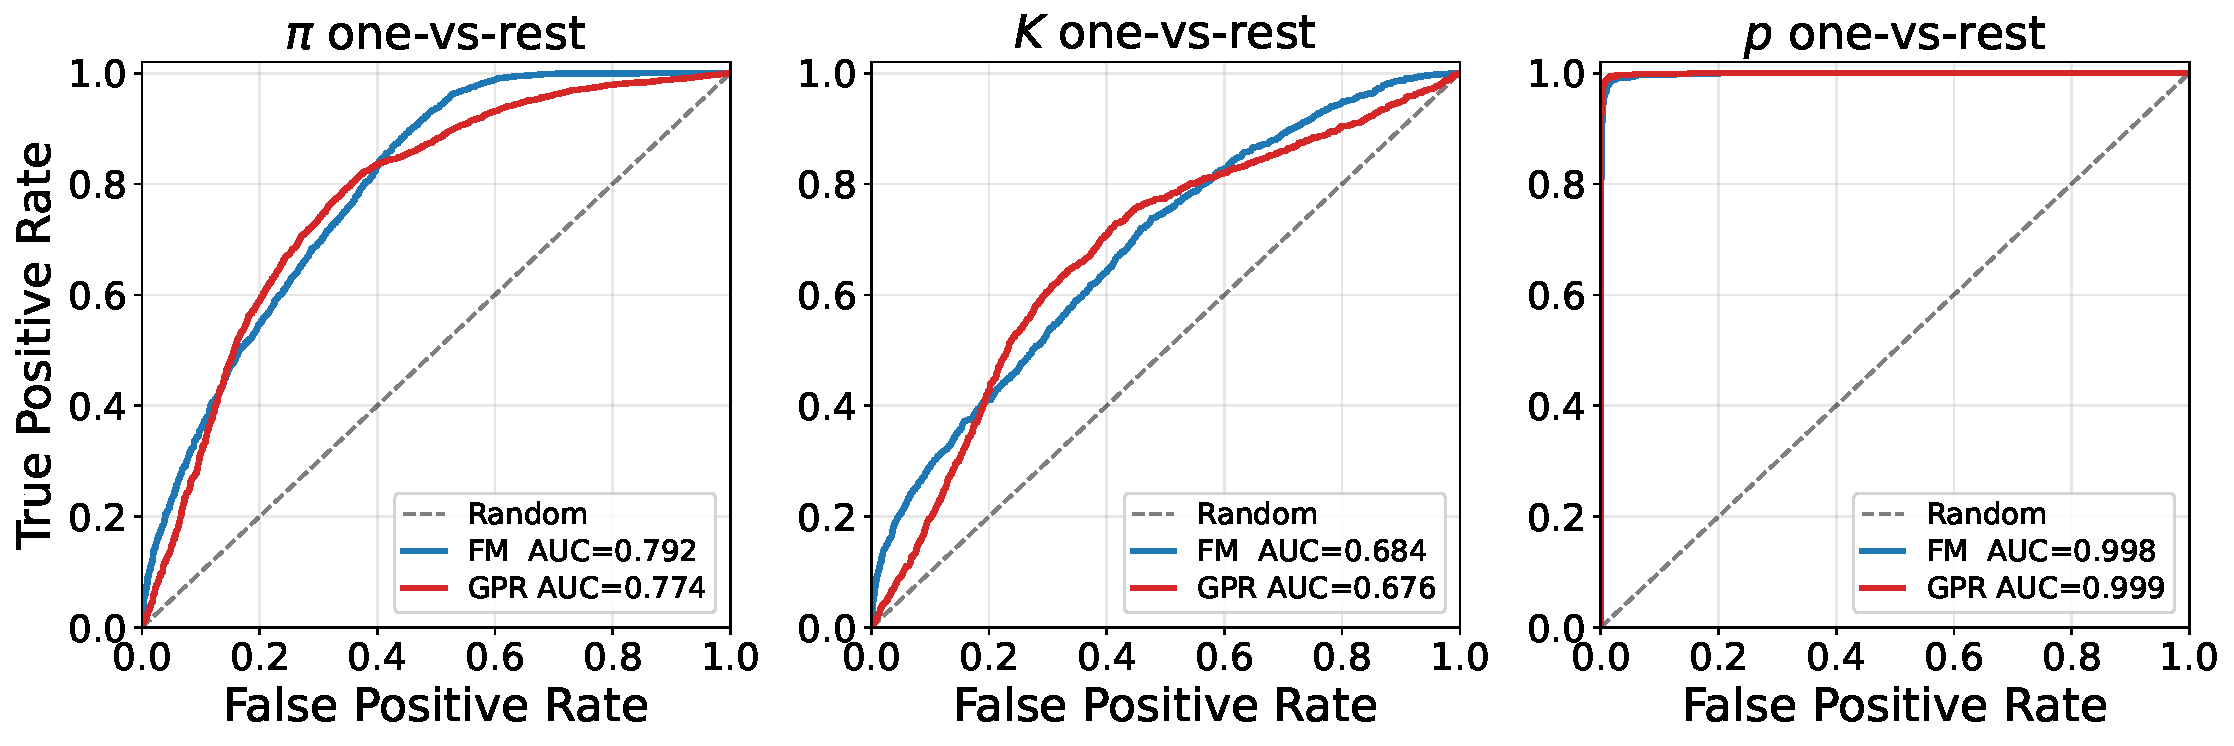
\includegraphics[width=\linewidth]{figures/pid_roc_0.8_1.2.pdf}
    \caption{One-vs-rest PID ROC curves for pions (left), kaons (middle), and protons (right) in the momentum slice $p \in [0.8, 1.2)$~GeV/$c$, comparing the FM4NPP model (blue) with the traditional GPR \dedx\ baseline (red). The dashed diagonal denotes random performance, and the area under each curve (AUC) is quoted in the legend. Both methods are evaluated on the same reconstructed tracks matched to primary particles. Tracks are charge-folded and the classification is restricted to the $\pi/K/p$ hypotheses for both methods.}
    \label{fig:pid_roc}
\end{figure*}

The track finding efficiency is shown in Fig.~\ref{fig:efficiency} for both the FM-based reconstruction and the traditional CA-based seeding algorithm. At relatively high $p_T$ both algorithms are quite efficient because the tracks are nearly straight in the magnetic field, making pattern recognition and track following simpler. However, at low $p_T$ ($p_T \lesssim 1.0$) the FM-based reconstruction significantly outperforms the traditional algorithm. Current track finding algorithms typically perform poorly at low $p_T$ due to larger effects of multiple scattering and a higher curvature of the track. Both effects result in pattern recognition becoming more difficult, since there are potentially large deflections of the track and the space points traverse larger regions in azimuth. Additionally, depending on the radial extent of the tracking system and the magnetic field strength, tracks begin to loop and leave nearly identical trajectories at multiple locations in z. Typical reconstruction algorithms are focused on maximizing performance in higher $p_T$ regimes above the threshold for these ``looper'' tracks. Efforts exist to develop standalone algorithms that are responsible for reconstructing loopers~\cite{Battisti:2024nqq}. The benefit of the FM is demonstrated in that a single architecture is capable of reconstructing tracks across the entire $p_T$ spectrum with extremely high efficiency. The training and architecture scheme of the FM are chosen in such a way to learn the patterns of all track momenta, since the same underlying physical principles apply across the full $p_T$ range.


Complementing the efficiency, the purity of the FM-based and CA-based seeding algorithms is shown in Fig.~\ref{fig:purity}. Both algorithms have a very high purity except at low $p_T$, where the CA seeder does not join consecutive loops for particles that loop within the sPHENIX magnetic field with high efficiency. In contrast, the FM has a purity of nearly unity even at low $p_T$ ($p_T \lesssim 0.5$). This shows that the FM finds the correct track and also that it does not duplicate tracks, even for low $p_T$ loopers, which may leave many bending track patterns along the $z$ axis in a single event within the TPC. 


The results of the PID separation are shown in Fig.~\ref{fig:pid_roc}. Protons are cleanly separated by both methods with an AUC $\geq 0.998$ for both, reflecting the large \dedx\ separation of protons from the lighter species in this momentum range. For pions the FM slightly outperforms the GPR baseline (AUC 0.792 versus 0.774), while for kaons---the most challenging case, as they sit between the pion and proton bands---the two methods are comparable, with the curves crossing and the FM area under the curve slightly higher (0.684 versus 0.676). The PID performance is primarily determined by the physical characteristics of the TPC; for example, a TPC with a larger radius and ionizing gas that liberates more electrons will have larger \dedx per track, improving the possibility of particle identification separation. The sPHENIX TPC was designed to mitigate effects from space charge distortions and not for PID performance. The FM performance being comparable to, and slightly better than, the traditional GPR performance is a powerful result when considered in the context of the FM pretraining objective focusing on track finding and spatial pattern recognition. Despite this, the FM learned features in the cluster correlations amongst the tracks to discern what the energy loss characteristics in the TPC were and was able to perform \dedx based separation comparably to the GPR method without explicit training. 



Several directions remain for future work. The FM studied here was trained using data from a single detector subsystem, whereas nuclear and particle physics experiments contain multiple subsystems that provide complementary information about reconstructed particles. An experiment-wide foundation model could incorporate information from tracking detectors, calorimeters, and other detector systems. For example, incorporating calorimeter information could enable the reconstruction of particle-flow-like objects that combine tracking and deposited-energy measurements. The broader FM4NPP roadmap identifies the development of AI-ready data infrastructure, scaling to larger and multimodal models, knowledge transfer across experiments and facilities, and the integration of scientific reasoning and tool-use capabilities as important future directions~\cite{Ren:2026fm4npproadmap}. Transfer learning across different physics domains has already shown promising results~\cite{Krzmanc:2026fdw}. Further studies using spacepoint data from other detectors, collision systems, and experimental conditions are needed to determine the generalizability of the learned representations. Furthermore, selecting pretraining objectives that are more generalizable, such as one that may include energy loss for particle identification, may improve the performance of the FM for a wider range of downstream tasks.

\section{Conclusions}
We have evaluated an FM-based approach to low-level particle reconstruction using simulated sPHENIX TPC data. The FM-based track-finding method substantially improves the reconstruction efficiency relative to the conventional Cellular Automaton-based method at low $p_T$ while maintaining high purity across the studied momentum range. The improvement is particularly pronounced for low-$p_T$ looping tracks, which are challenging for conventional reconstruction algorithms. At higher $p_T$, both methods achieve similarly high tracking efficiency and purity.

The same frozen pretrained backbone can also support particle identification through a supervised downstream adapter. The FM-based particle identification method achieves performance similar to that of the conventional GPR-based \dedx{} method for kaons and protons in the selected momentum interval, and slightly better pion discrimination. Notably, the pretraining objective did not explicitly involve energy or ionization-energy-loss prediction. These results indicate that a shared pretrained backbone could support several reconstruction tasks using appropriate downstream adapters, potentially simplifying data analysis and extending the reach of measurements, particularly at low $p_T$.
%We have shown that a FM-based approach to low level particle reconstruction can have dramatically improved downstream results when compared to traditional algorithms. Furthermore, a single model can provide comparable or better performance for multiple downstream tasks, simplifying data analysis and potentially enabling new measurements previously inaccessible especially at low $p_T$. These results suggest that pretraining identifies kinematic correlations beyond those for which the architecture is designed, indicating that a single model could be used for several downstream tasks given the relevant input data. Additionally, there are real performance benefits that can arise from utilizing modern AI based algorithms to perform particle physics data reconstruction, as demonstrated by the significantly improved efficiency and purity compared to traditional methods. While traditional algorithms rely on assumptions about the expected shape of reconstructed tracks, we have shown a FM-based approach is capable of identifying the patterns that may depend on kinematics like $p_T$ and can thus perform well across a wide kinematic range. These results provide support for expanding available datasets to train new AI-based approaches for data reconstruction.


% Several directions remain for future work. The FM analyzed here was trained only on data from a single subsystem, while typical high energy nuclear and particle physics experiments contain up to dozens of subsystems. A complete FM would be trained on data from an entire experiment, which provides complementary information about the characteristics of the reconstructed particles. For example, adding in calorimeter data could enable deposited energy to be included in training and potentially particle-flow like four vectors to be reconstructed by the FM. This would naturally suit the multi-modal data that FMs are typically trained on. Furthermore, there have already been studies exploring the transfer learning capabilities of FMs~\cite{Krzmanc:2026fdw}. Additional studies including or testing the performance on other experimental spacepoint data to identify whether or not similar performance metrics can be achieved are warranted.



% If in two-column mode, this environment will change to single-column
% format so that long equations can be displayed. Use
% sparingly.
%\begin{widetext}
% put long equation here
%\end{widetext}

% figures should be put into the text as floats.
% Use the graphics or graphicx packages (distributed with LaTeX2e)
% and the \includegraphics macro defined in those packages.
% See the LaTeX Graphics Companion by Michel Goosens, Sebastian Rahtz,
% and Frank Mittelbach for instance.
%
% Here is an example of the general form of a figure:
% Fill in the caption in the braces of the \caption{} command. Put the label
% that you will use with \ref{} command in the braces of the \label{} command.
% Use the figure* environment if the figure should span across the
% entire page. There is no need to do explicit centering.

% \begin{figure}
% \includegraphics{}%
% \caption{\label{}}
% \end{figure}

% Surround figure environment with turnpage environment for landscape
% figure
% \begin{turnpage}
% \begin{figure}
% \includegraphics{}%
% \caption{\label{}}
% \end{figure}
% \end{turnpage}

% tables should appear as floats within the text
%
% Here is an example of the general form of a table:
% Fill in the caption in the braces of the \caption{} command. Put the label
% that you will use with \ref{} command in the braces of the \label{} command.
% Insert the column specifiers (l, r, c, d, etc.) in the empty braces of the
% \begin{tabular}{} command.
% The ruledtabular enviroment adds doubled rules to table and sets a
% reasonable default table settings.
% Use the table* environment to get a full-width table in two-column
% Add \usepackage{longtable} and the longtable (or longtable*}
% environment for nicely formatted long tables. Or use the the [H]
% placement option to break a long table (with less control than 
% in longtable).
% \begin{table}%[H] add [H] placement to break table across pages
% \caption{\label{}}
% \begin{ruledtabular}
% \begin{tabular}{}
% Lines of table here ending with \\
% \end{tabular}
% \end{ruledtabular}
% \end{table}

% Surround table environment with turnpage environment for landscape
% table
% \begin{turnpage}
% \begin{table}
% \caption{\label{}}
% \begin{ruledtabular}
% \begin{tabular}{}
% \end{tabular}
% \end{ruledtabular}
% \end{table}
% \end{turnpage}

% Specify following sections are appendices. Use \appendix* if there
% only one appendix.
%\appendix
%\section{}

% If you have acknowledgments, this puts in the proper section head.
%\begin{acknowledgments}
% put your acknowledgments here.
%\end{acknowledgments}

% Create the reference section using BibTeX:
\bibliography{bibliography.bib}

\end{document}
%
% ****** End of file apstemplate.tex ******

